%! Author = lili
%! Date = 8/12/26
\section{Abgabe 1.4}\label{sec:abgabe-1.4}

\subsection{HA 1.4.1}\label{subsec:ha-1.4.1}
Sei $(\Omega,P)$ ein Wahrscheinlichkeitsraum.

\begin{auf}[(a) Die Ereignisse $A,B,C,D\subseteq\Omega$ seien unabhängig. Beweisen Sie:]
    $\ $
    \begin{enumerate}
        \item $A\cap B$ und $C$ sind unabhängig.
        \item $A\cup B$ und $C\setminus D$ sind unabhängig.
    \end{enumerate}
    NOCH KEINE LÖSUNG % TODO NOCH KEINE LÖSUNG
\end{auf}

Sei $B\subseteq\Omega$ ein Ereignis mit $P(B)\in\{0,1\}$. Außerdem sei $A\subseteq\Omega$ ein beliebiges weiteres Ereignis.

\begin{auf}[(b) Zeigen Sie, dass $A$ und $B$ unabhängig sind.]
    $\ $
    \begin{figure}[H]
        \centering
        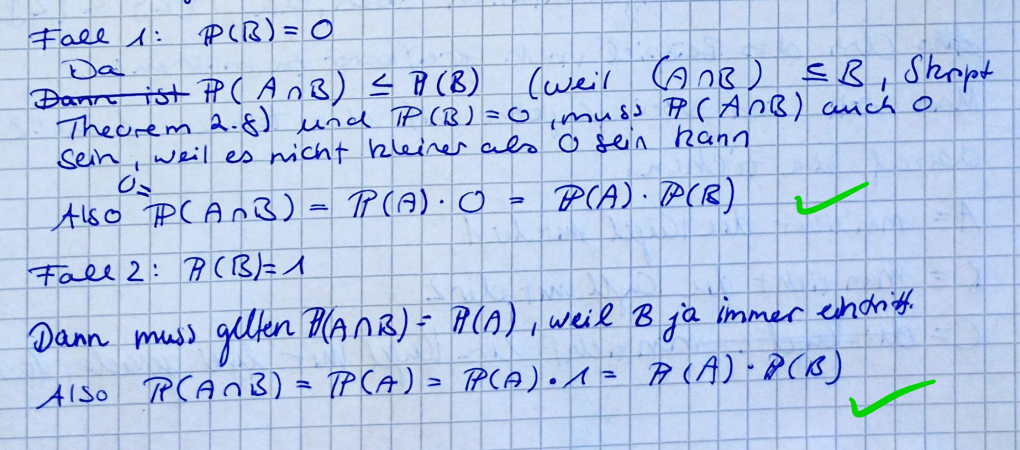
\includegraphics[width=0.8\linewidth]{images/lösungen/wts141b}
    \end{figure}
    \textit{ Beachten Sie: $P(B)\in\{0,1\}$ impliziert nicht, dass $B=\varnothing$ oder $B=\Omega$ gilt.}
\end{auf}

Es seien Ereignisse $A,B,C\subseteq\Omega$ gegeben. Dabei gelte sowohl, dass $A\cap B$ und $C$ unabhängig sind, als auch, dass $A\cup B$ und $C$ unabhängig sind.

\begin{auf}[(c) Geben Sie ein Beispiel an, das zeigt, dass $A,B$ und $C$ nicht unabhängig sein müssen.]
    $\ $ \\
    NOCH KEINE LÖSUNG % TODO NOCH KEINE LÖSUNG
    \textit{Hinweis:} Es gibt ein einfaches Beispiel mit einem Ereignisraum mit nur zwei Elementen.
\end{auf}

\subsection{HA 1.4.2 \abhaken}
Seien $X$ und $Y$ zwei Zufallsvariablen mit einer gemeinsamen Dichte $f:\mathbb R^2\to[0,\infty)$, gegeben durch
\[
    f(x,y) = \begin{cases}
                 c\,xy^2 & \text{falls } 0\le x\le y\le 1, \\
                 0 & \text{sonst},
    \end{cases}
\]
mit $c\in\mathbb R$.
\begin{auf}[(a) Bestimmen Sie $c\in\mathbb R$ so, dass $f$ eine Dichte ist.]
    $\ $
    \begin{figure}[H]
        \centering
        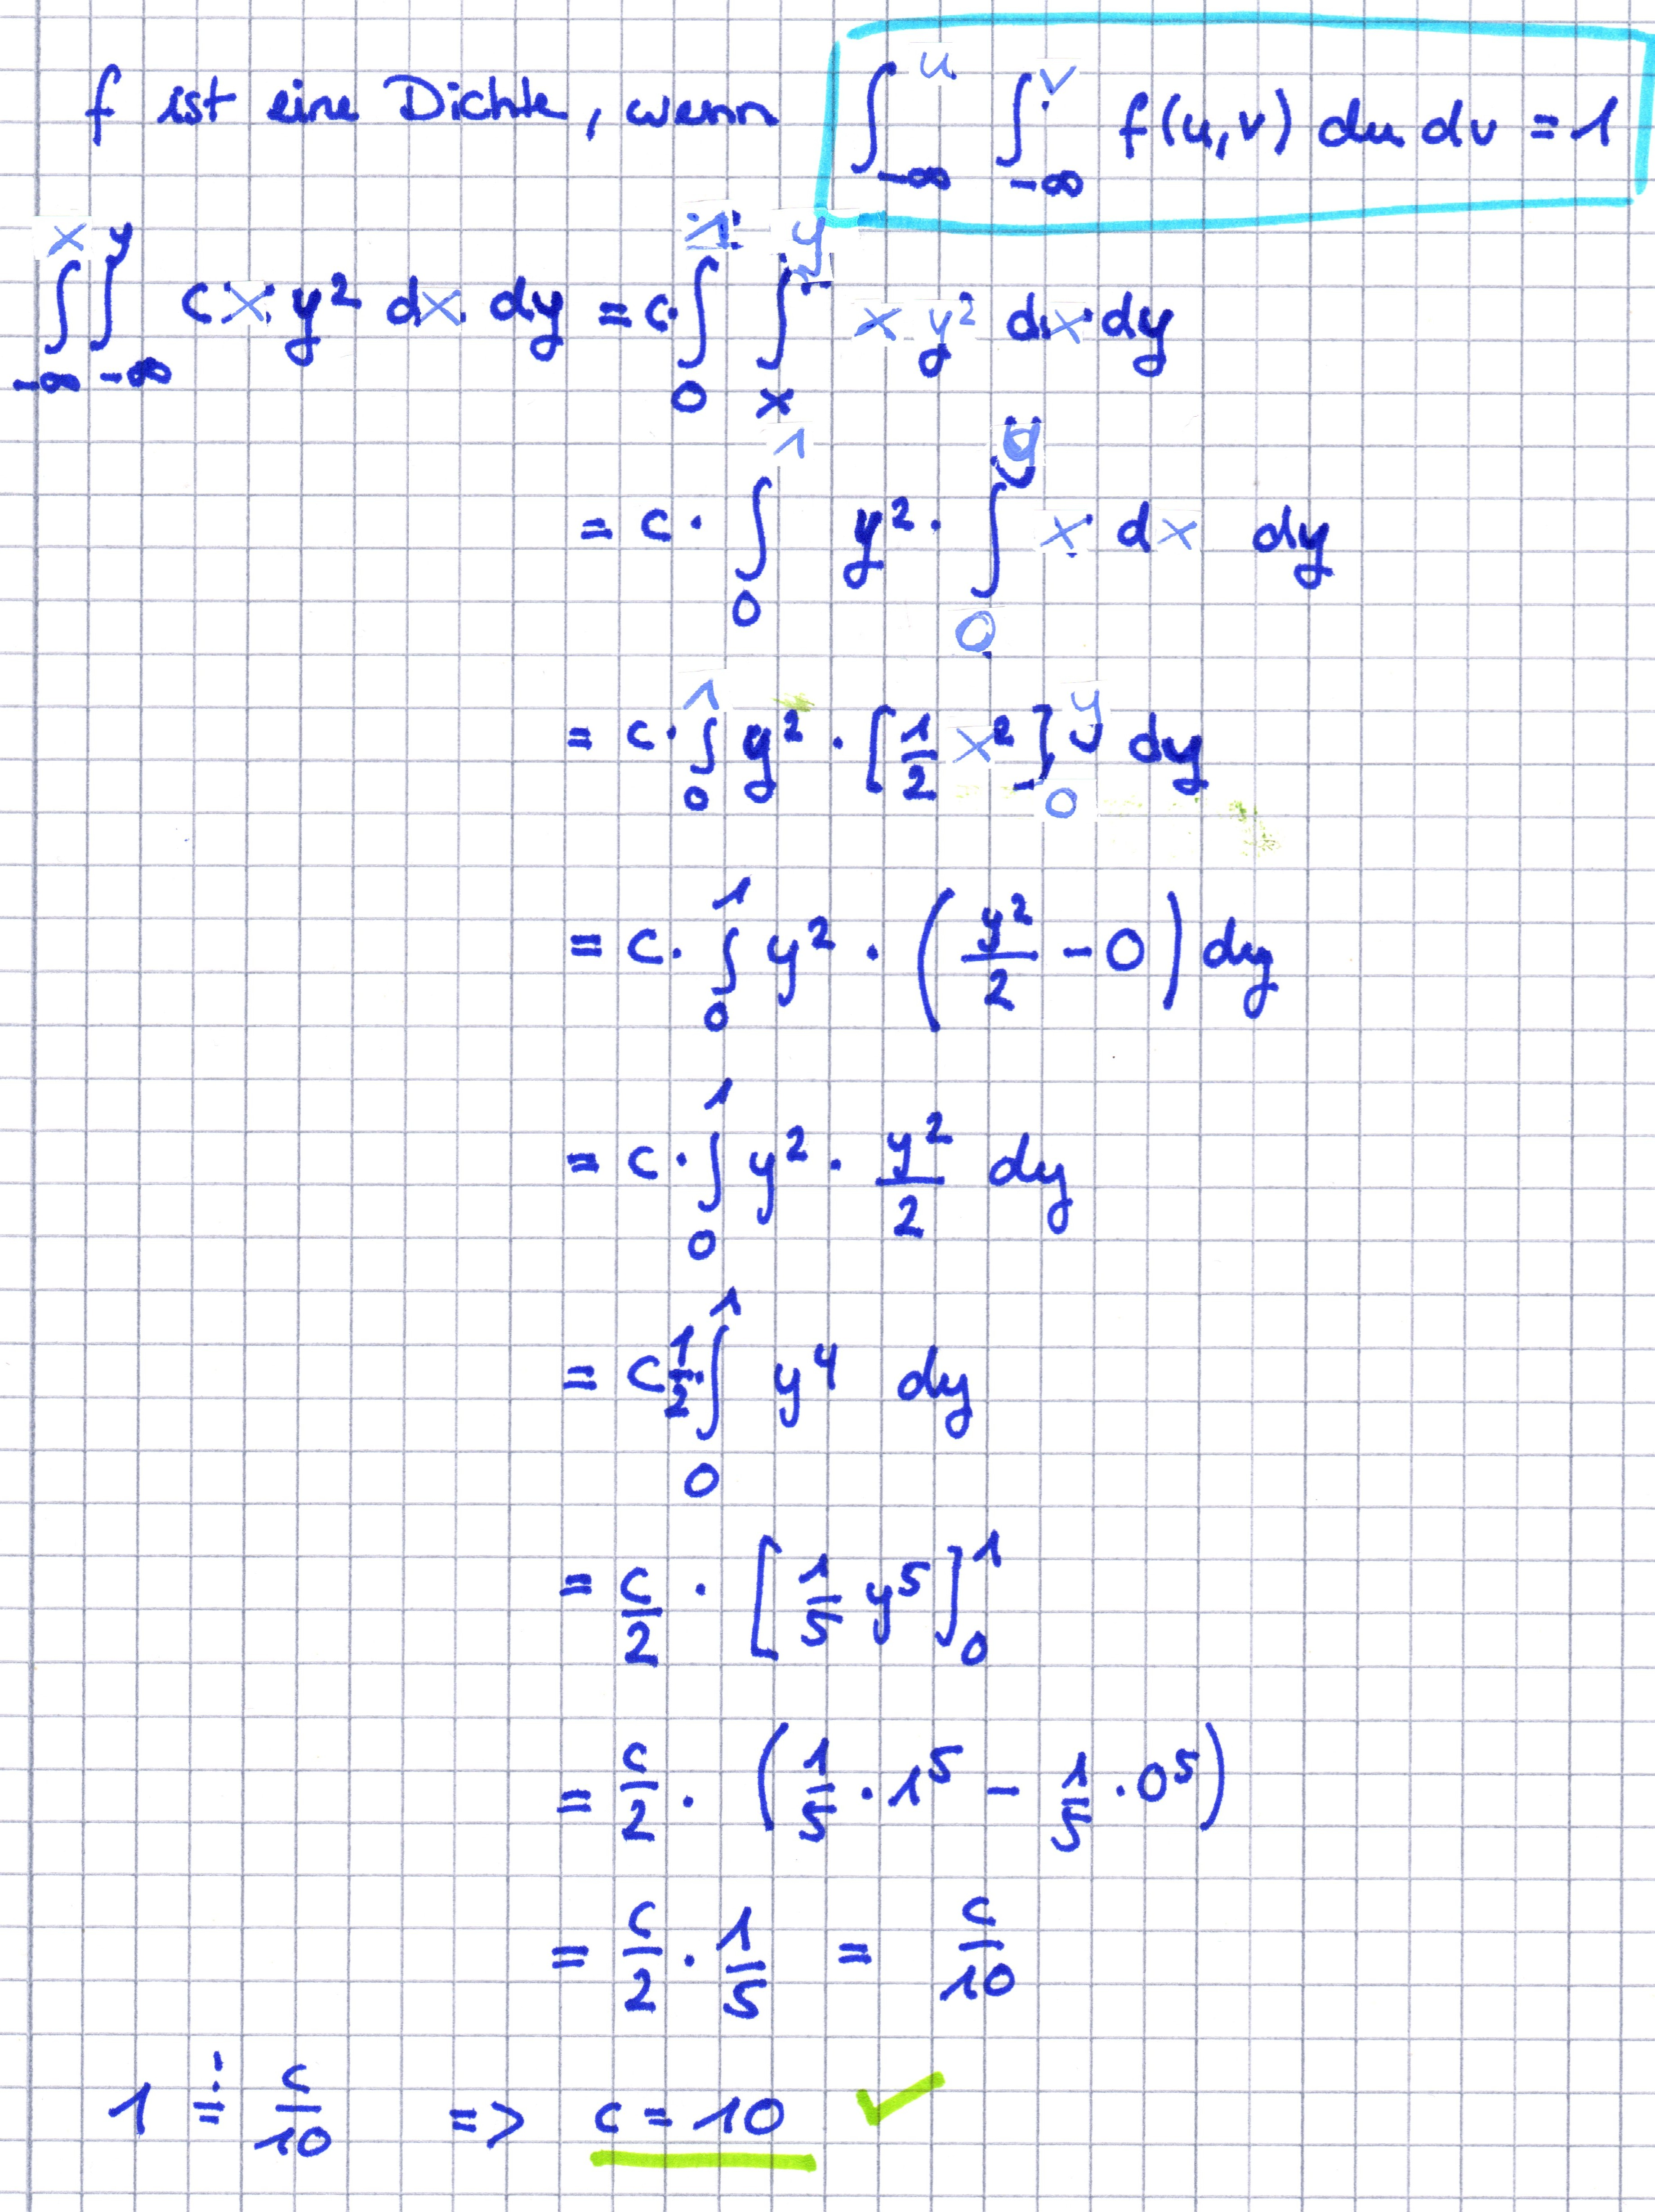
\includegraphics[width=0.8\linewidth]{images/lösungen/wts142a}
    \end{figure}
\end{auf}

\begin{auf}[(b) Berechnen Sie $P(2X>Y)$. \textit{Hinweis:} Skizzieren Sie zunächst den Integrationsbereich.]
    $\ $
    \begin{figure}[H]
        \centering
        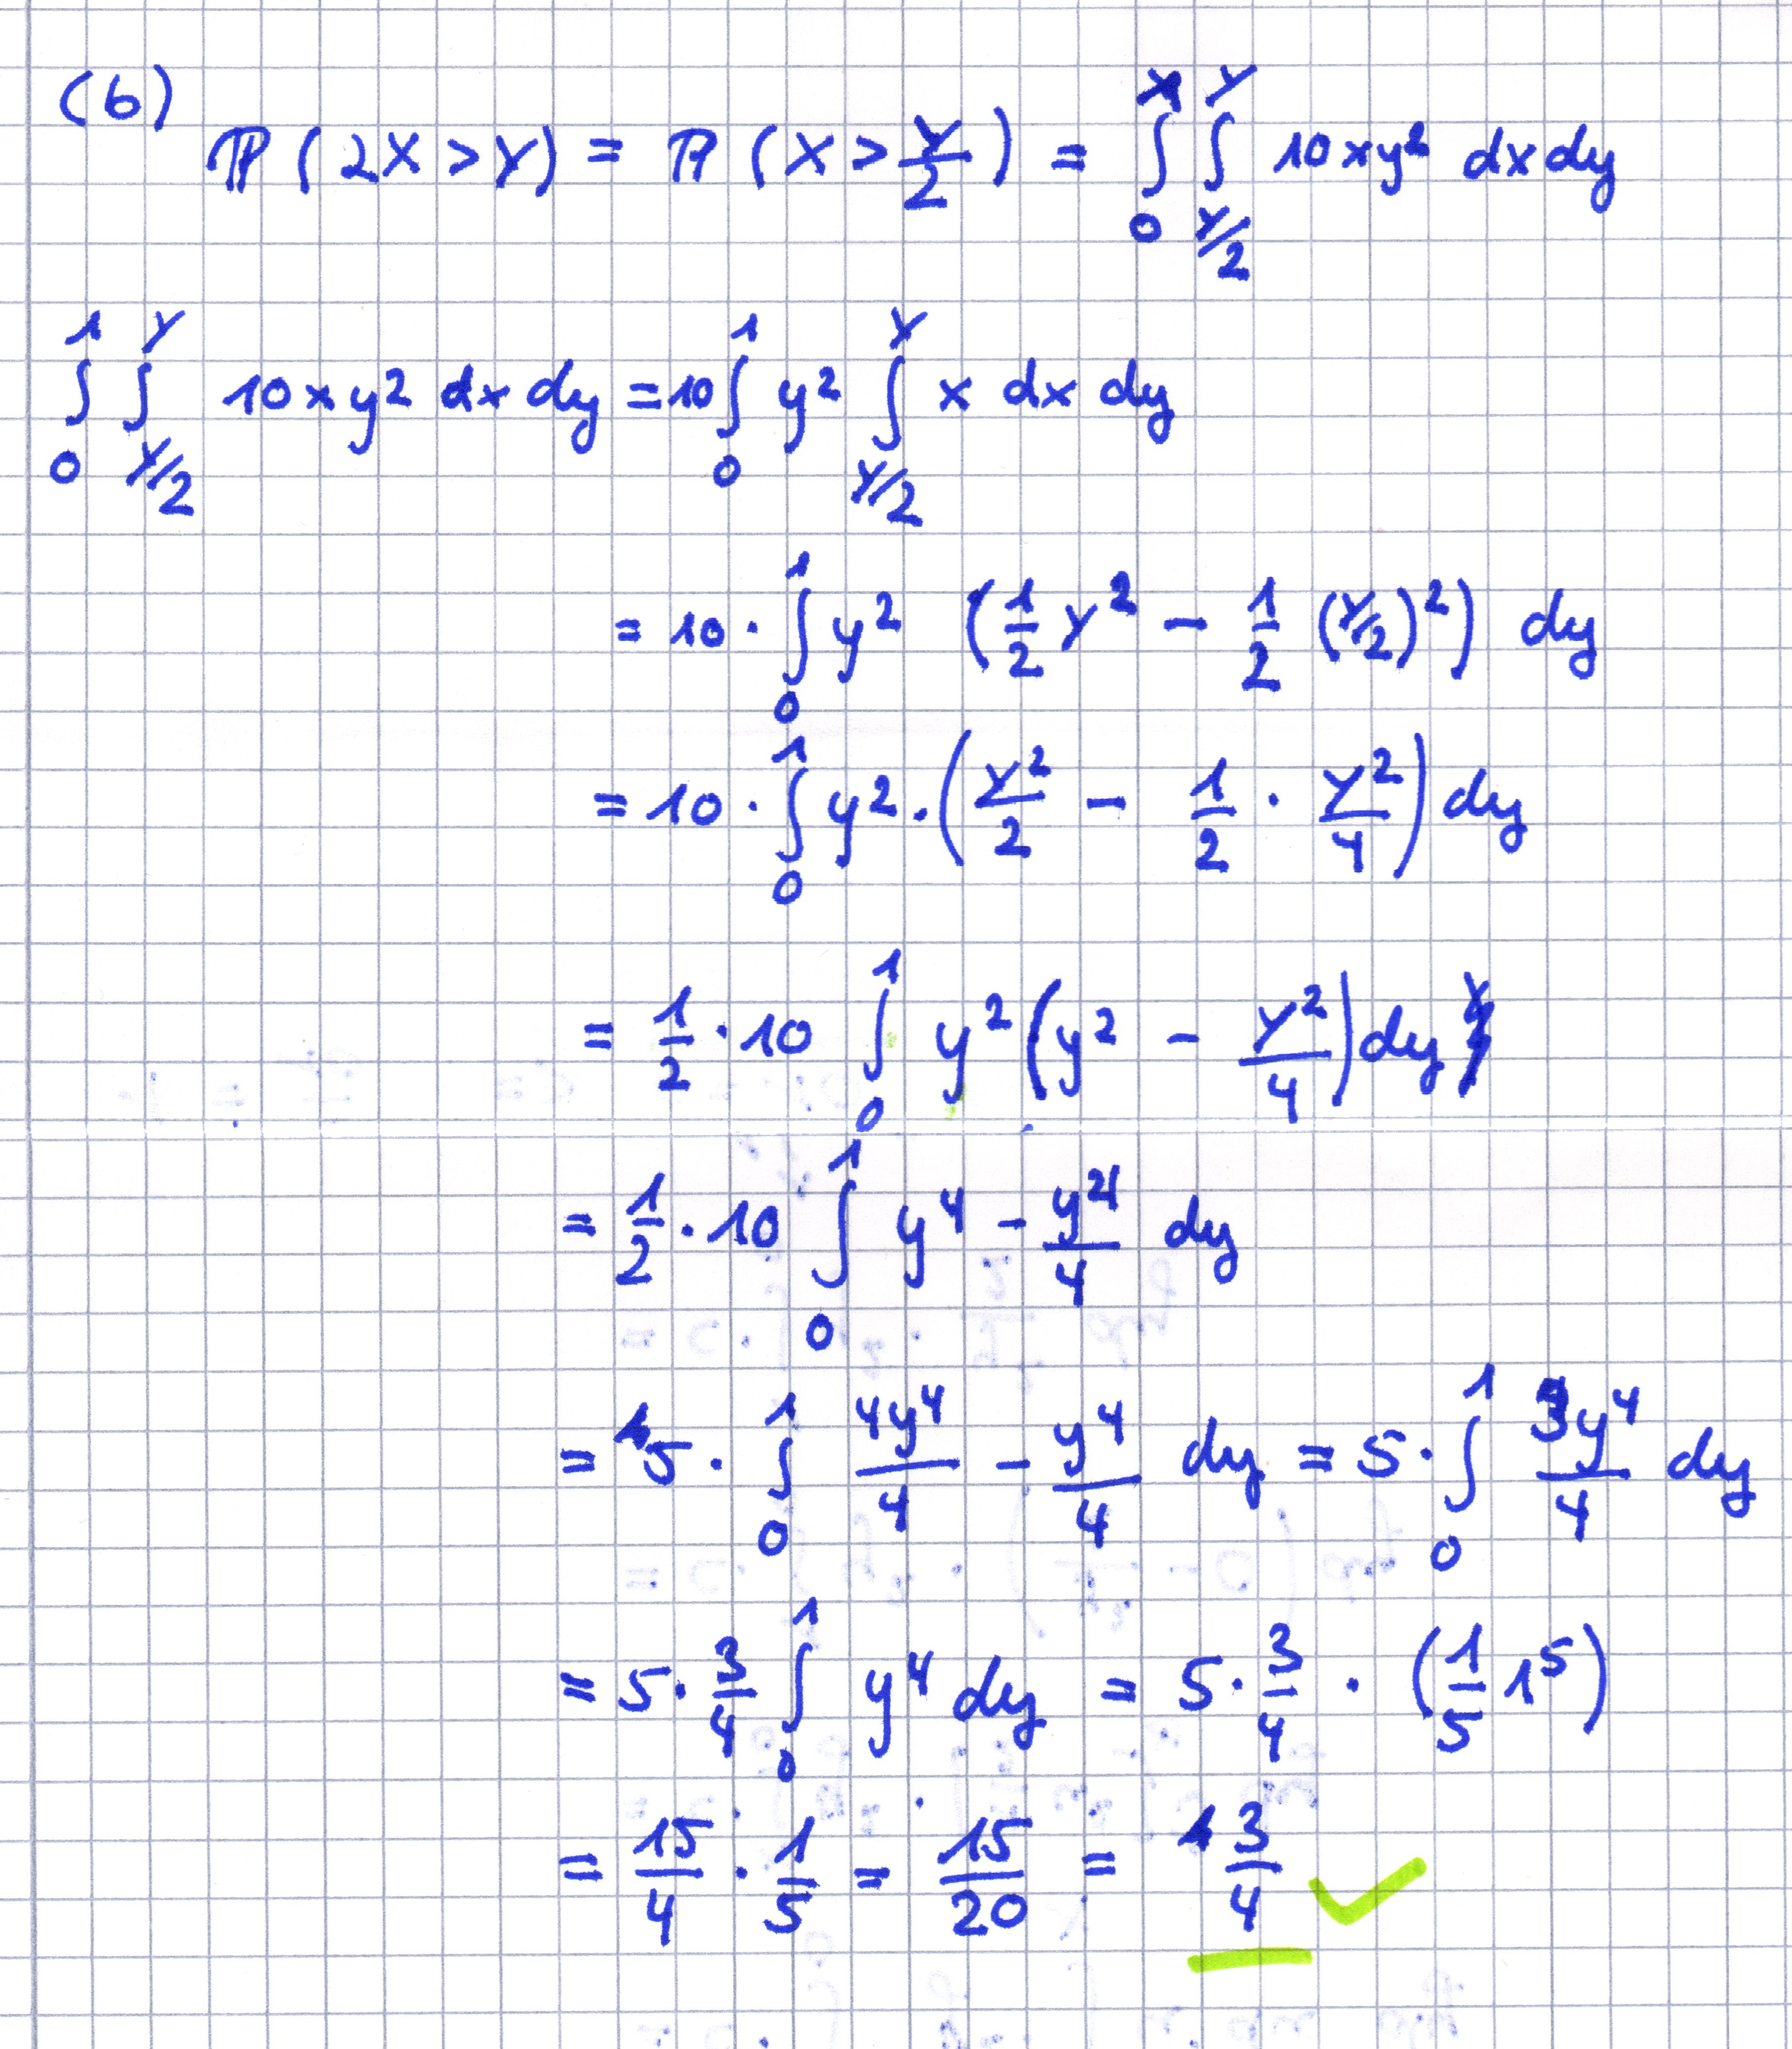
\includegraphics[width=0.8\linewidth]{images/lösungen/wts142b}
    \end{figure}
\end{auf}

\begin{auf}[(c) Bestimmen Sie die Randdichten von $X$ und $Y$.]
    $\ $
    \begin{figure}[H]
        \centering
        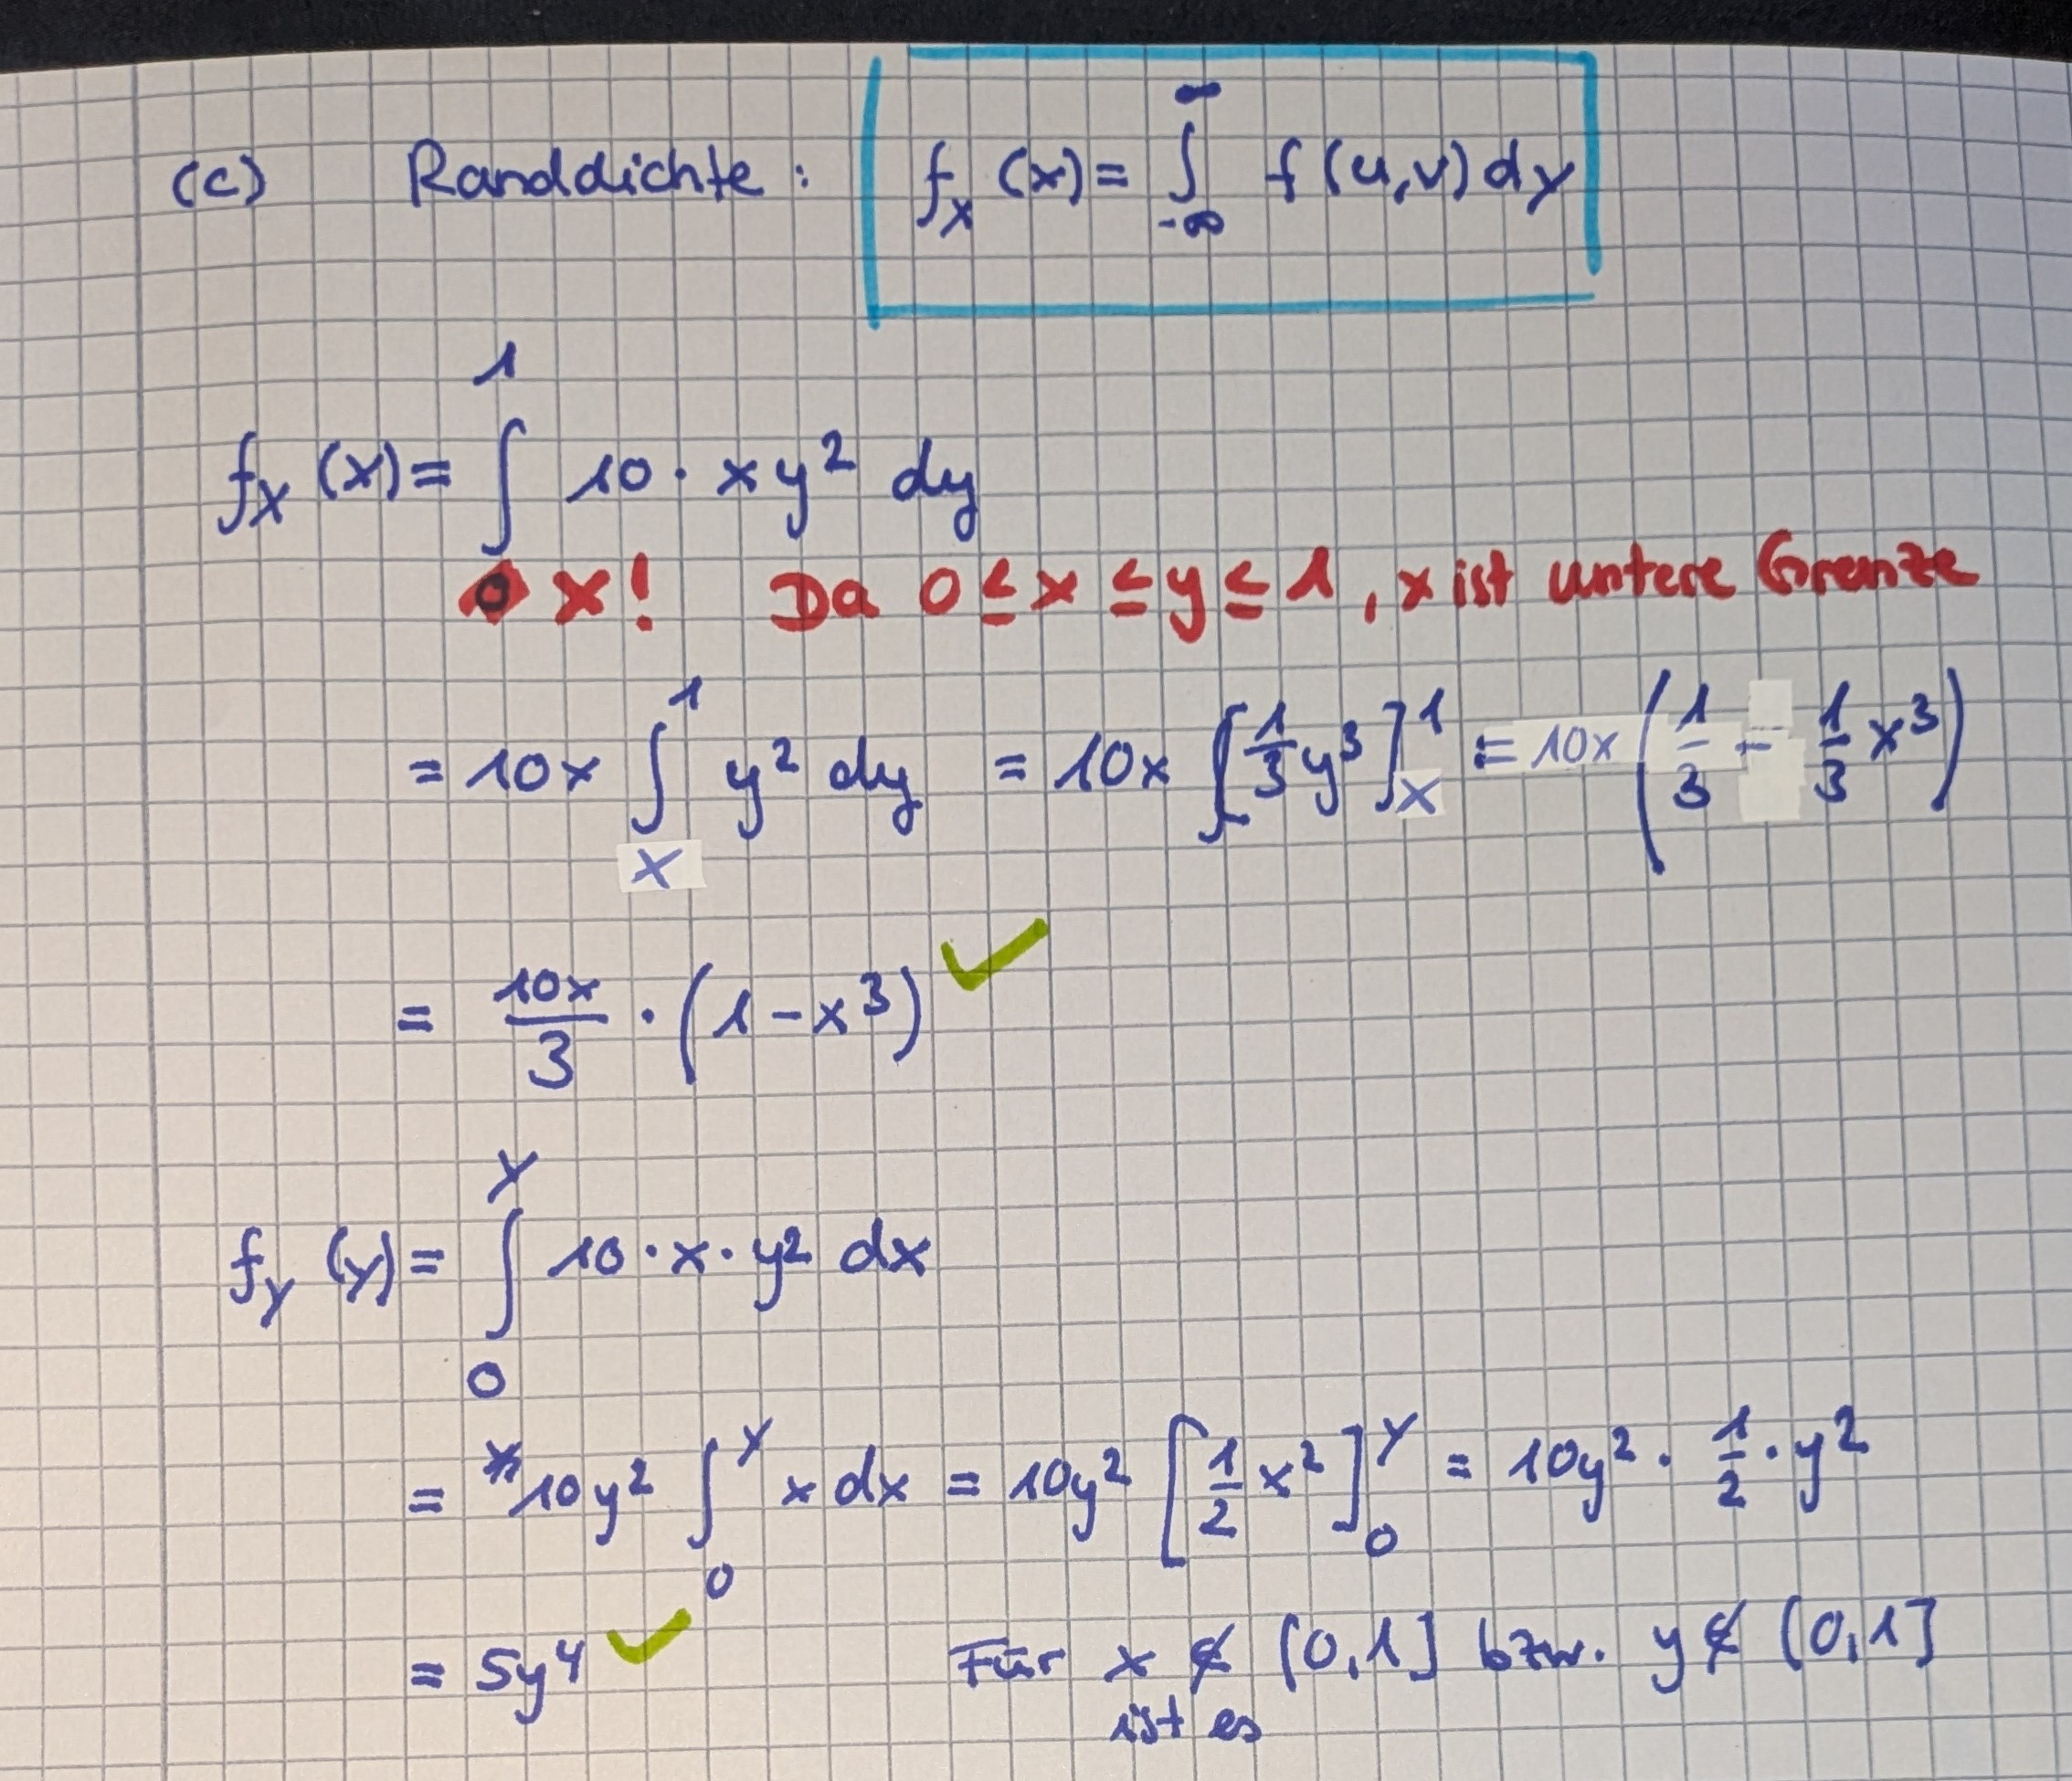
\includegraphics[width=0.8\linewidth]{images/lösungen/wts142c}
    \end{figure}
\end{auf}

\begin{auf}[(d) Bestimmen Sie die Verteilungsfunktionen von $X$ und $Y$.]
    $\ $
    \begin{figure}[H]
        \centering
        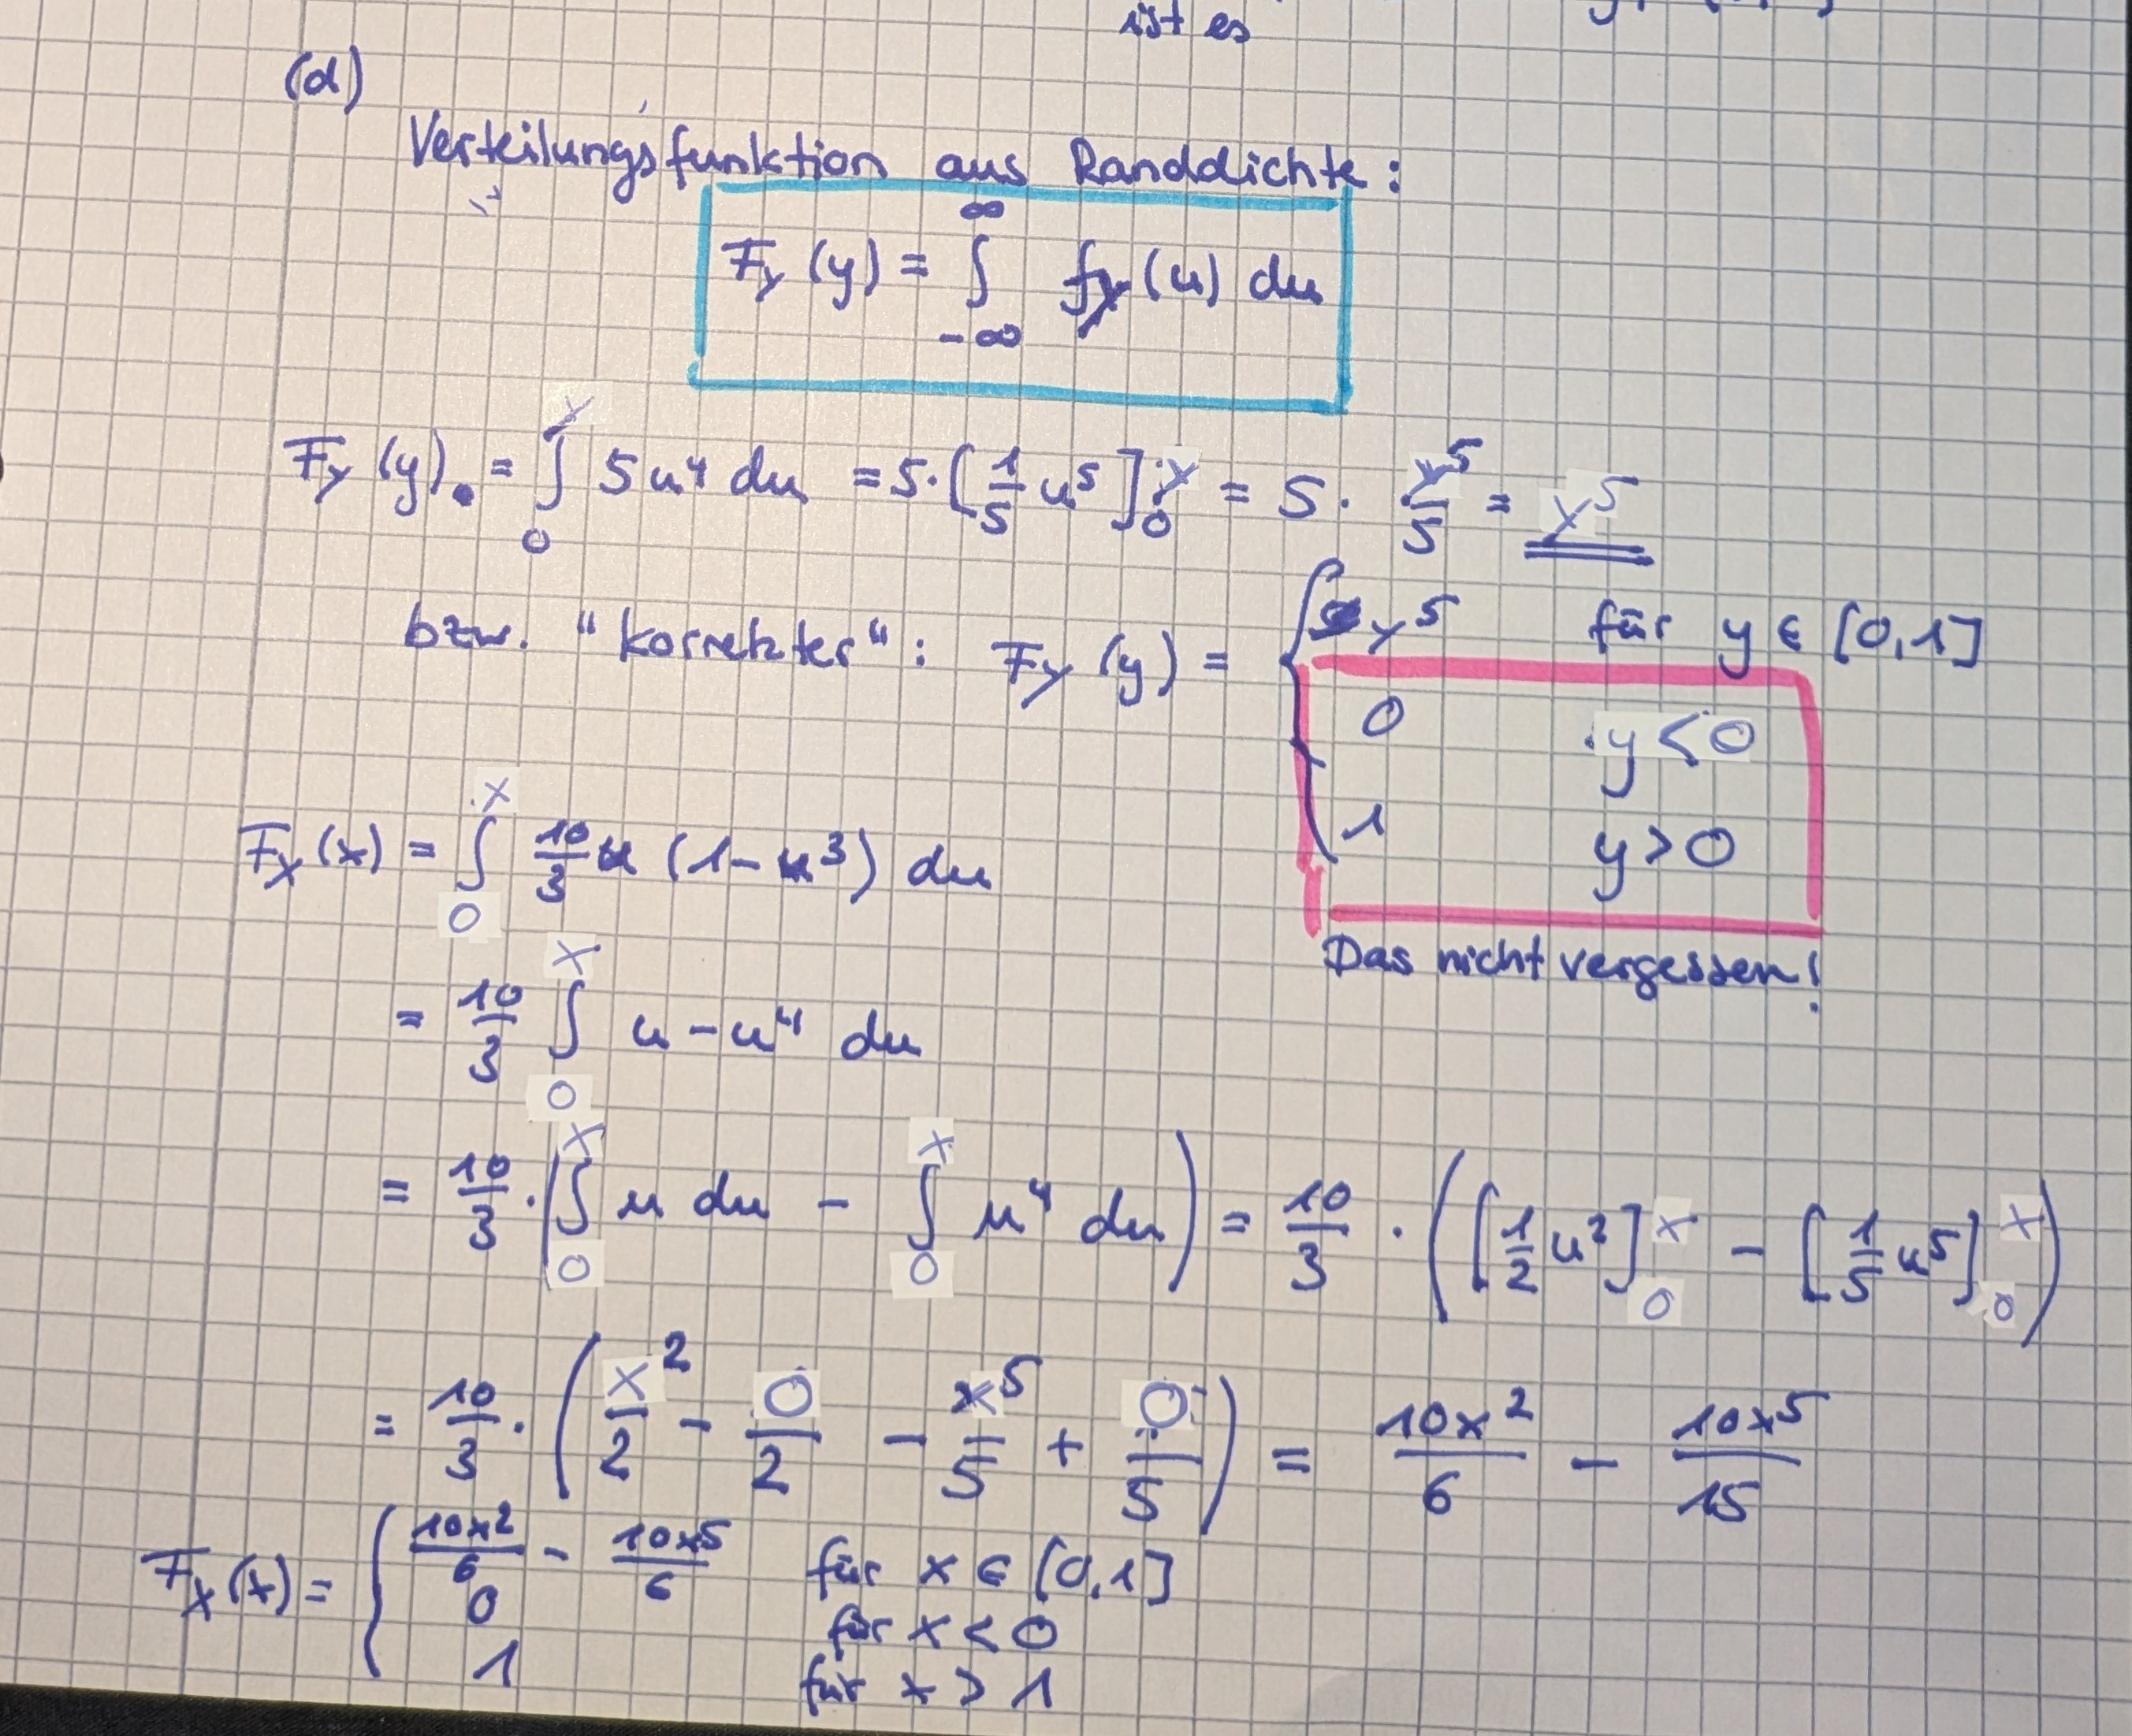
\includegraphics[width=0.8\linewidth]{images/lösungen/wts142d}
    \end{figure}
\end{auf}


\begin{auf}[(e) Sind die Ereignisse $\{X\le a\}$ und $\{Y\le b\}$ für alle $a,b\in\mathbb R$ unabhängig? Beweisen Sie Unabhängigkeit oder zeigen Sie, dass die Ereignisse für eine konkrete Wahl von $a,b\in\mathbb R$ nicht unabhängig sind.]
    $\ $
    \begin{figure}[H]
        \centering
        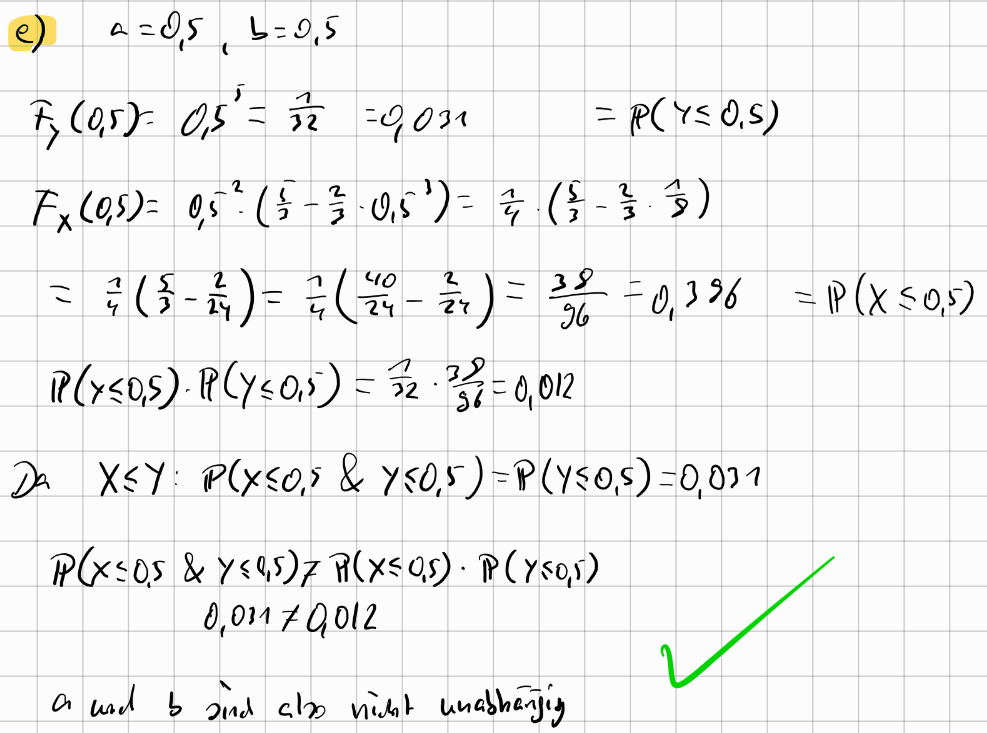
\includegraphics[width=0.8\linewidth]{images/lösungen/wts142e}
    \end{figure}
\end{auf}

\subsection{HA 1.4.3 \abhaken}\label{subsec:ha-1.4.3}
Eine Multiple-Choice-Klausur bestehe aus $N=4K$ Fragen, von denen jede nur richtig oder falsch beantwortet werden kann. Die Klausur ist bestanden, wenn mindestens $2K$ Fragen richtig bearbeitet wurden. René nimmt an der Klausur teil. Leider hat er einen schlechten Tag und beantwortet daher jede einzelne der Fragen, unabhängig von allen anderen Fragen, nur mit einer Wahrscheinlichkeit von 60\% richtig.

\begin{auf}[(a) Geben Sie einen geeigneten Wahrscheinlichkeitsraum $(\Omega,P)$ an, der es erlaubt, die folgenden Aufgabenteile zu bearbeiten.]
    $\ $
    \begin{figure}[H]
        \centering
        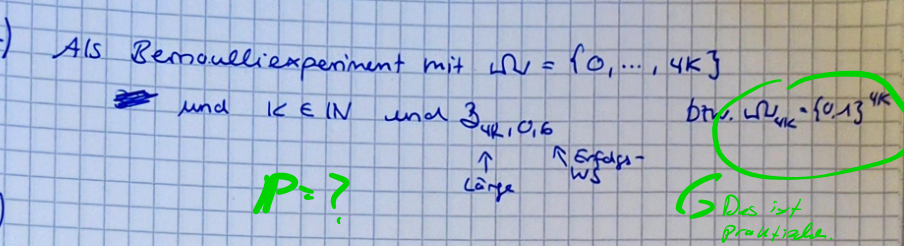
\includegraphics[width=0.8\linewidth]{images/lösungen/wts143a}
        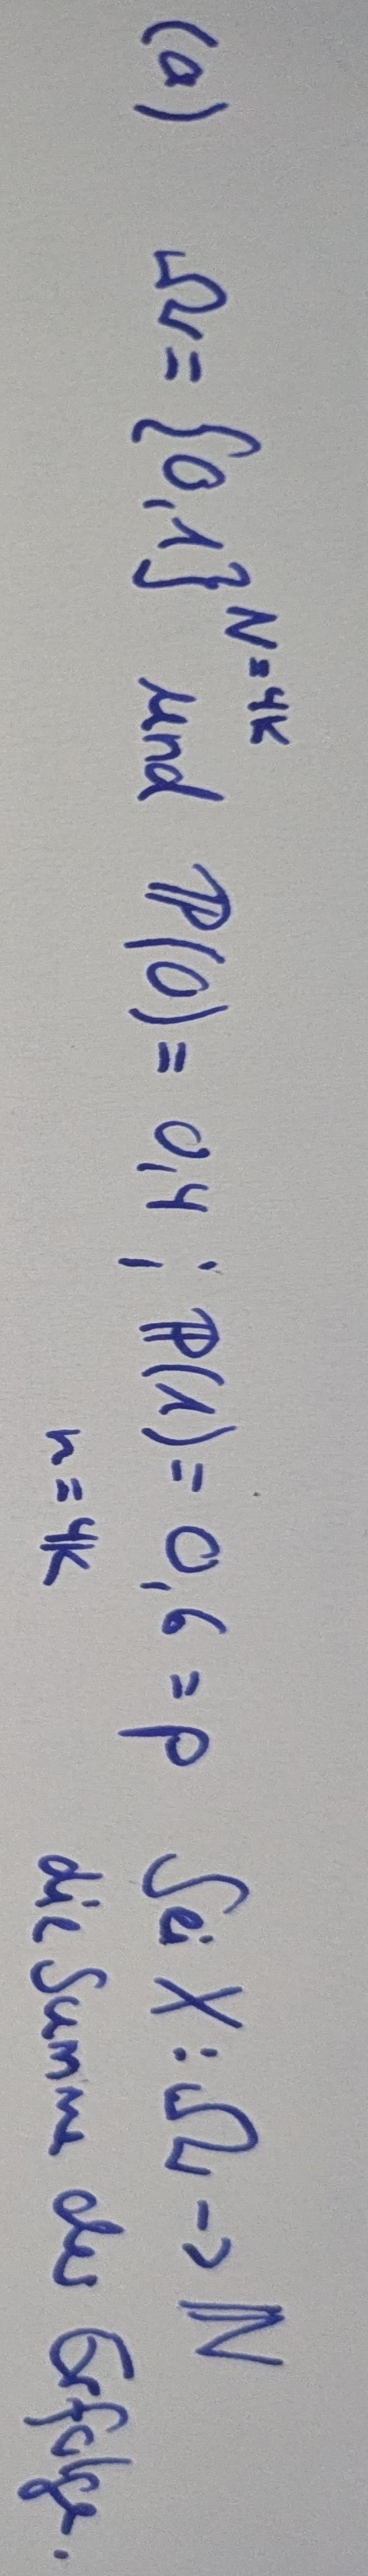
\includegraphics[width=0.8\linewidth]{images/lösungen/wts143a-2}
    \end{figure}
\end{auf}

\begin{auf}[(b) Bestimmen Sie die Wahrscheinlichkeit, dass René die Klausur besteht.]
    $\ $
    \begin{figure}[H]
        \centering
        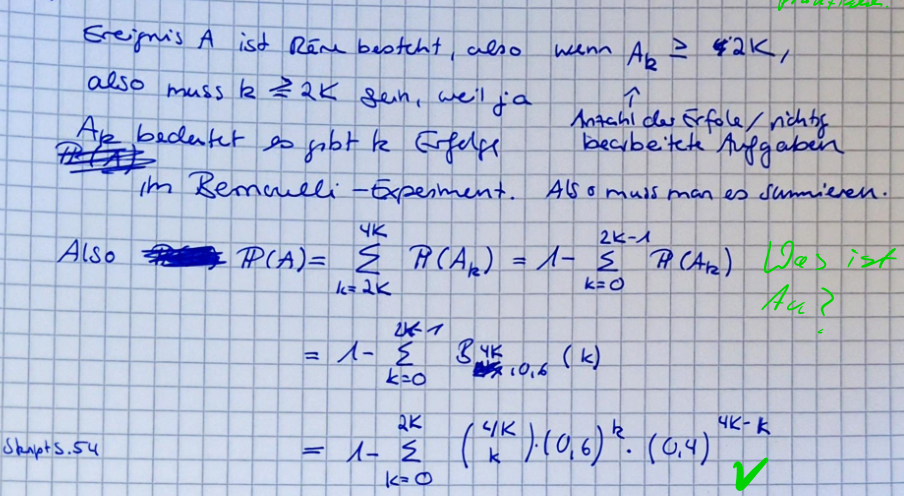
\includegraphics[width=0.8\linewidth]{images/lösungen/wts143b}
        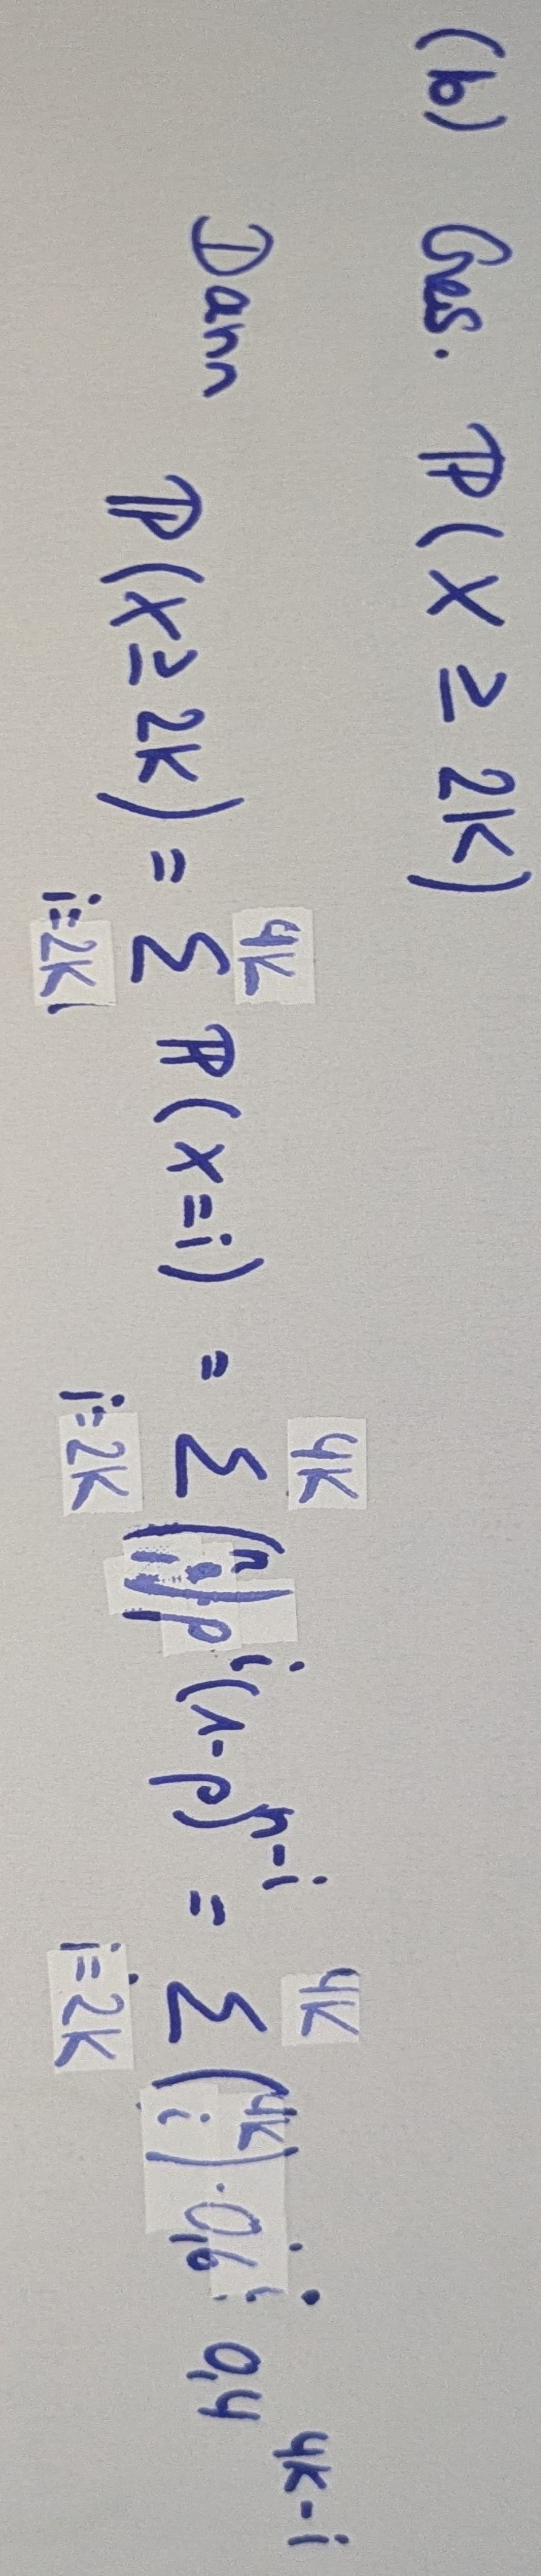
\includegraphics[width=0.8\linewidth]{images/lösungen/wts143b-2}
    \end{figure}
\end{auf}

\begin{auf}[(c) Das richtige Beantworten von $3K$ Fragen genügt für die Note 2,3. Bestimmen Sie die Wahrscheinlichkeit, dass René mindestens die Note 2,3 erreicht.]
    $\ $
    \begin{figure}[H]
        \centering
        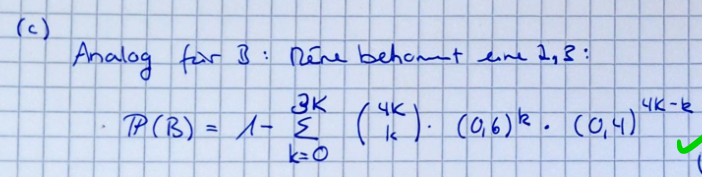
\includegraphics[width=0.8\linewidth]{images/lösungen/wts143c}
        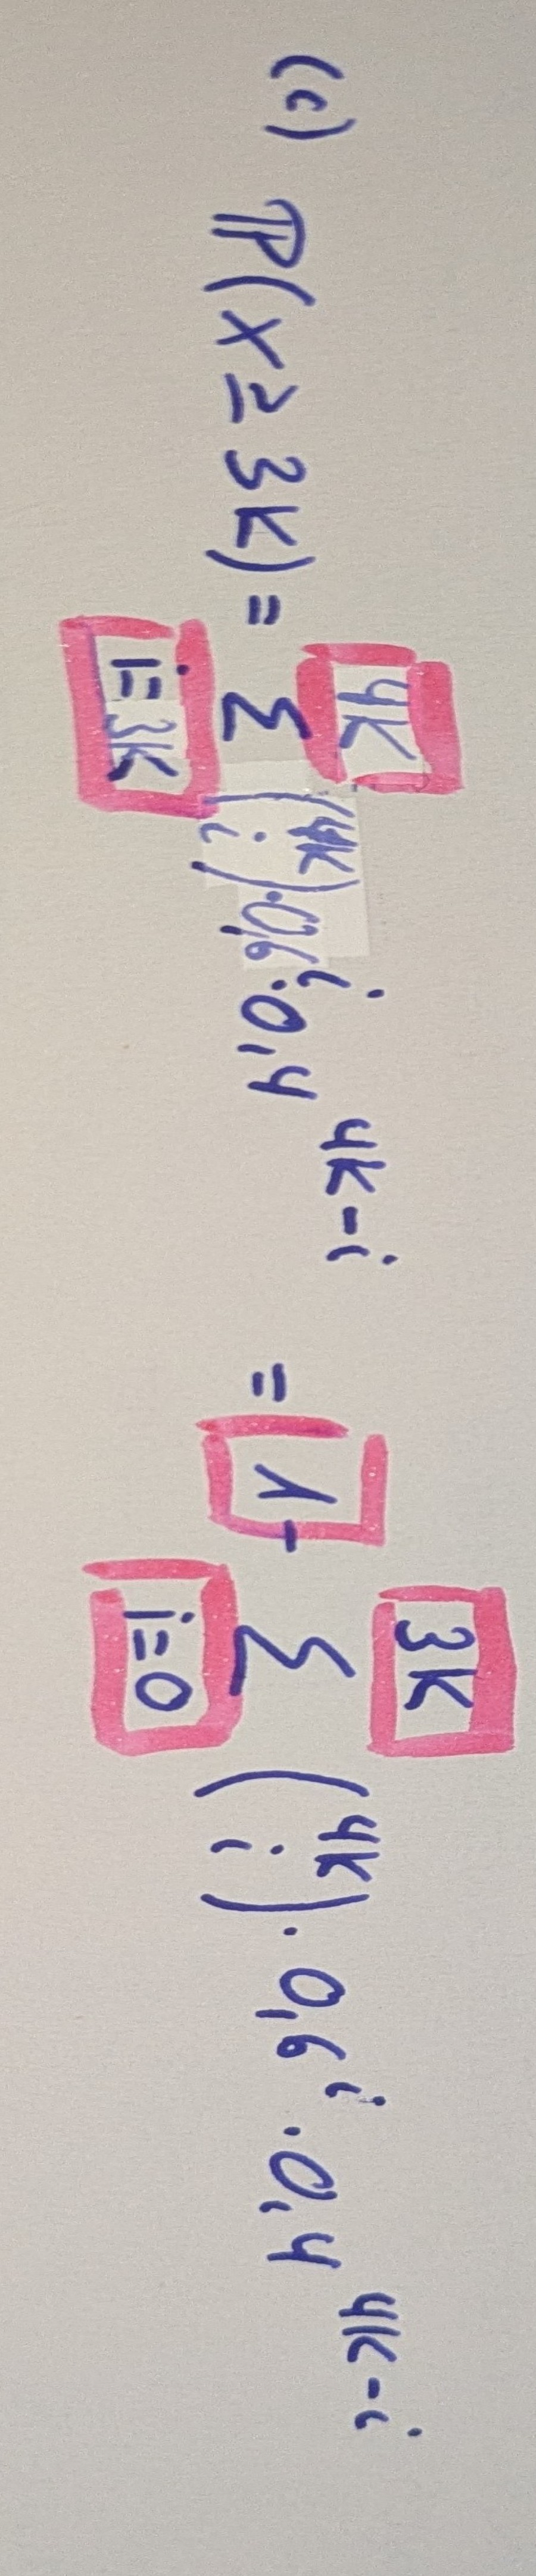
\includegraphics[width=0.8\linewidth]{images/lösungen/wts143c-2}
    \end{figure}
\end{auf}


\begin{auf}[(d) Geben Sie die Werte für die Wahrscheinlichkeit, dass René mindestens die Note 2,3 erreicht, explizit an für $K=5$, $K=10$ und $K=20$.]
    $\ $
    \begin{figure}[H]
        \centering
        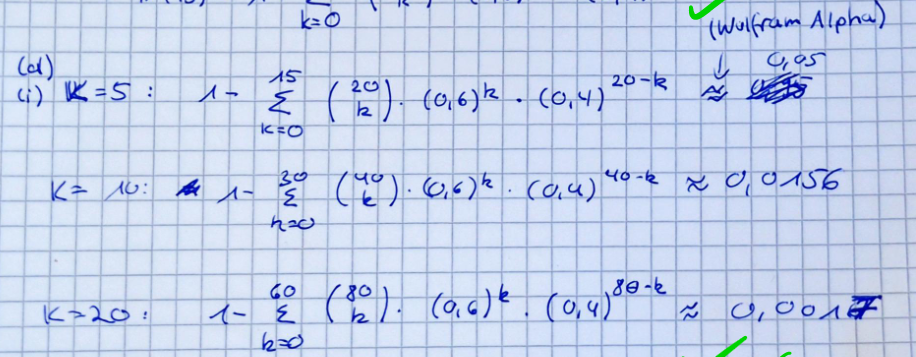
\includegraphics[width=0.8\linewidth]{images/lösungen/wts143d}
        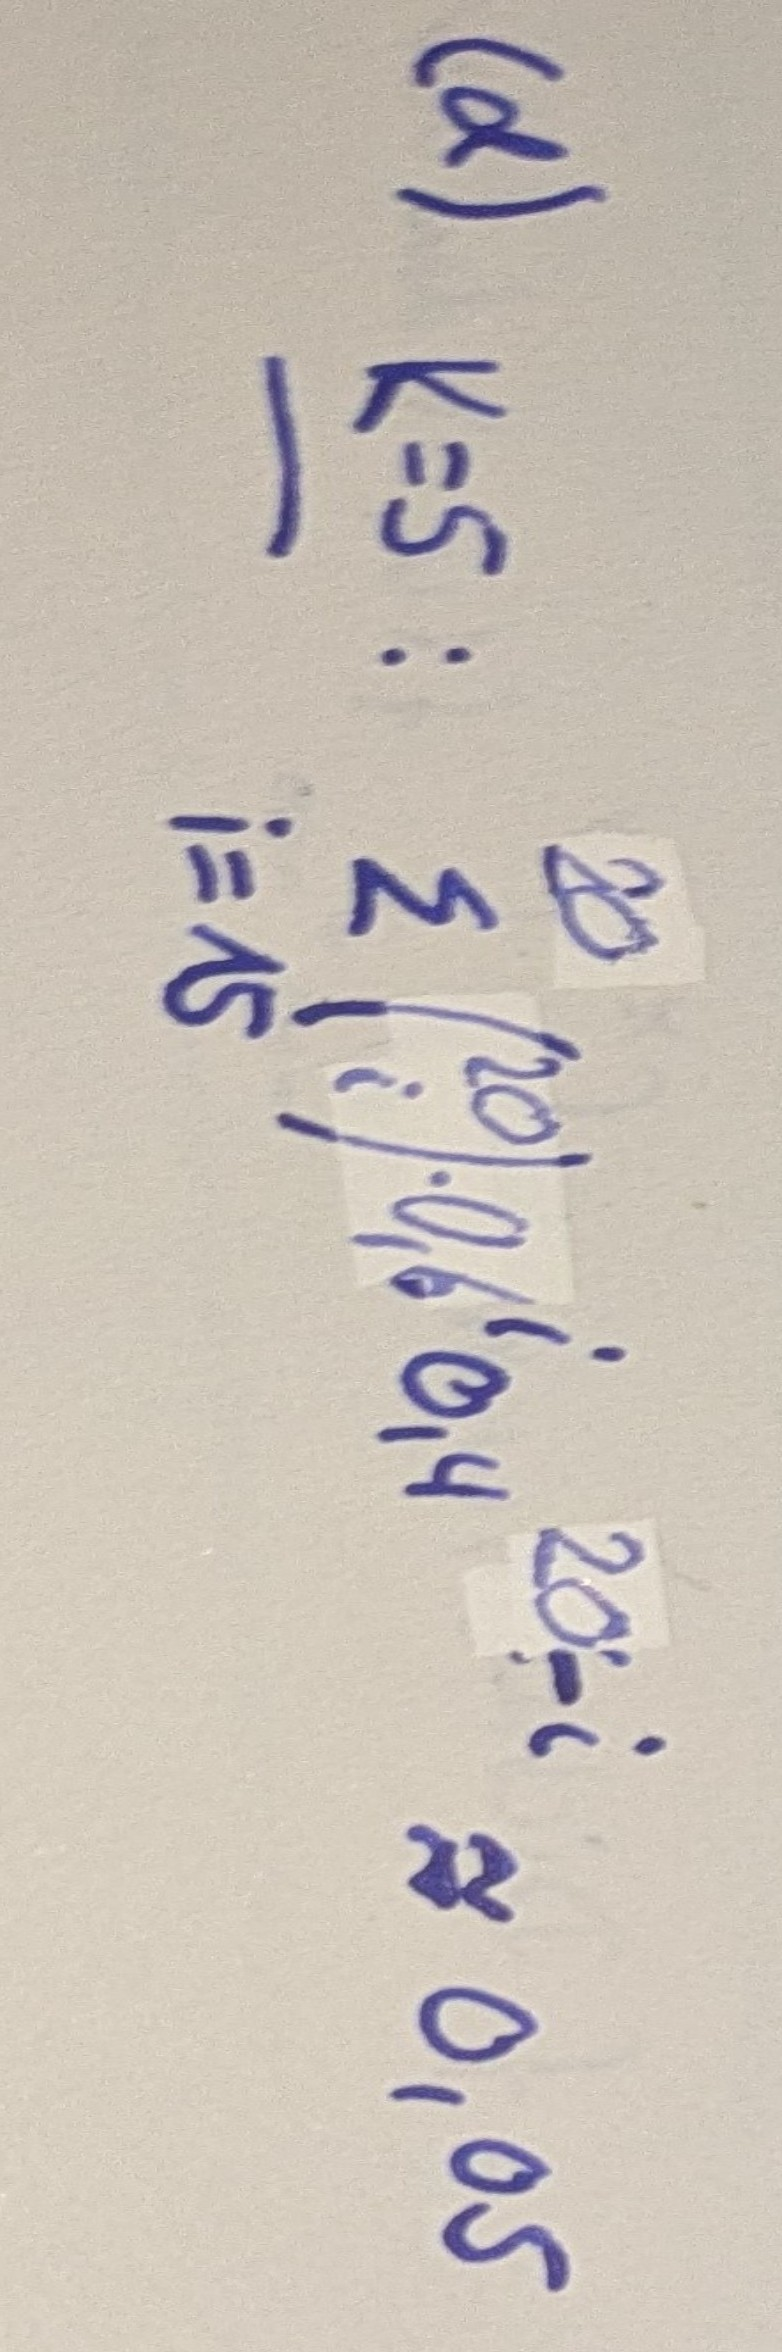
\includegraphics[width=0.8\linewidth]{images/lösungen/wts143d-2}
    \end{figure}
\end{auf}